\section{Results}
\label{sec:results}

We got those results.

We calculate $\mathrm{B}(\muF)$, $\deltaQCD(\muR,\muF)$ and 
$\deltaEW(\muF^0)$

\subsection{\texorpdfstring{$\boldsymbol pp\to \gamma\gamma\gamma$}{pp->aaa}}

\begin{figure}[t!]
  \centering
  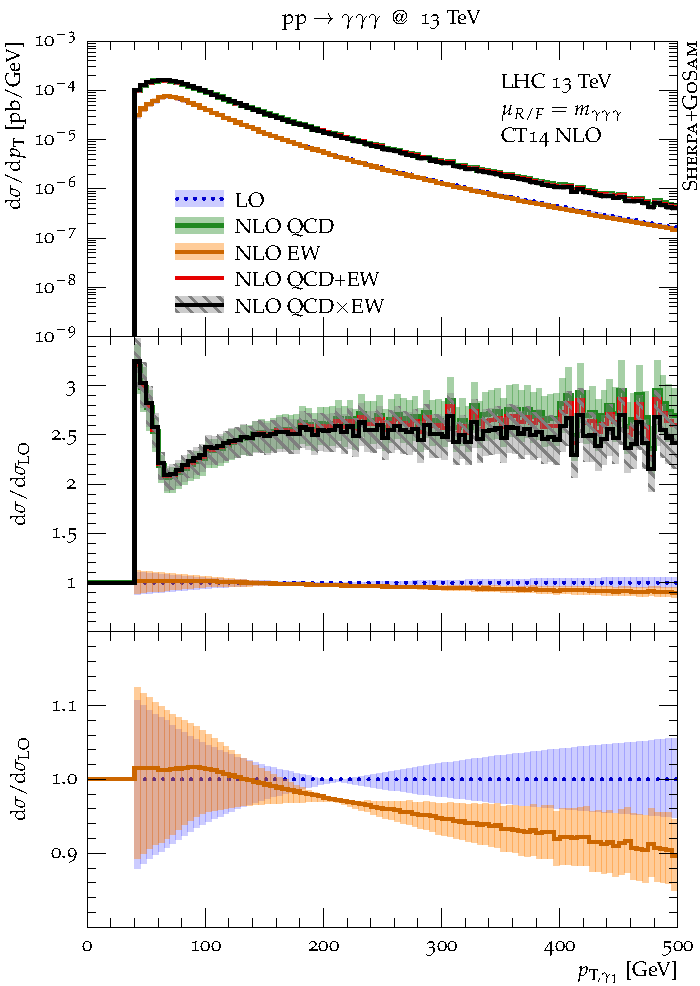
\includegraphics[width=0.32\textwidth]{figs_aaa/pT_y1}
  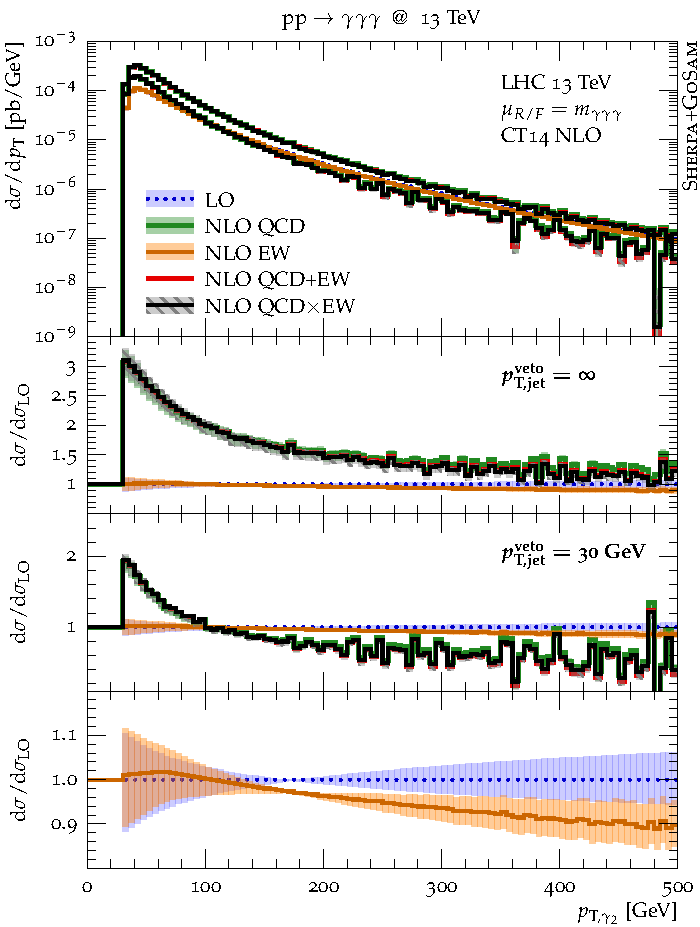
\includegraphics[width=0.32\textwidth]{figs_aaa/pT_y2}
  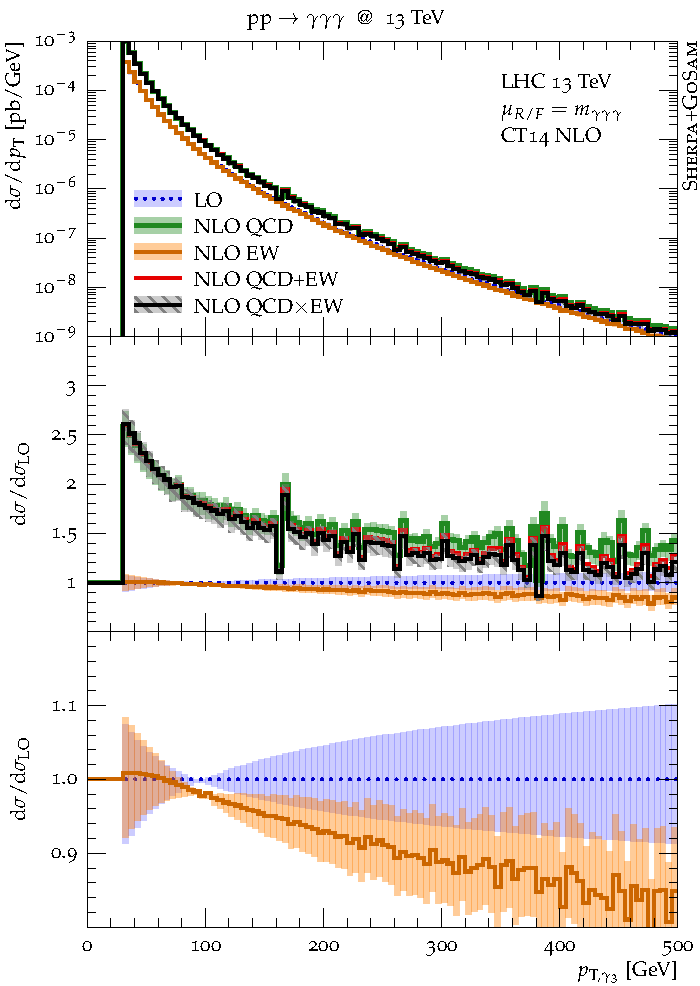
\includegraphics[width=0.32\textwidth]{figs_aaa/pT_y3}
  \caption{
    Transverse momentum of the leading (left), subleading (centre) 
    and third leading (right) photon at the LHC at 13\,TeV.
    \label{fig:aaa:pt}
  }
\end{figure}

\begin{figure}[t!]
  \centering
  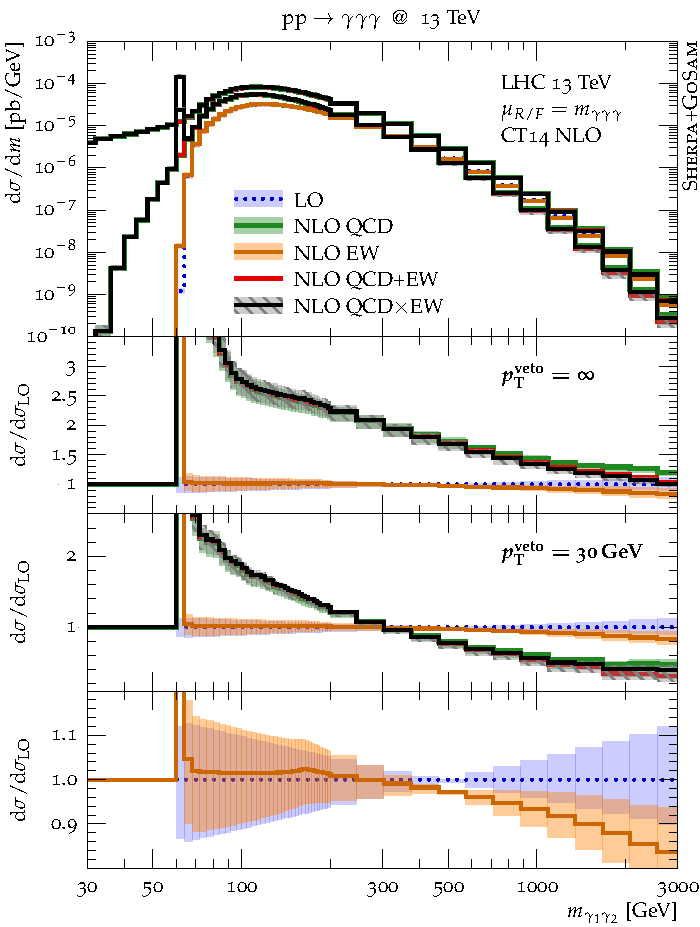
\includegraphics[width=0.32\textwidth]{figs_aaa/m_y1y2_comb_log}
  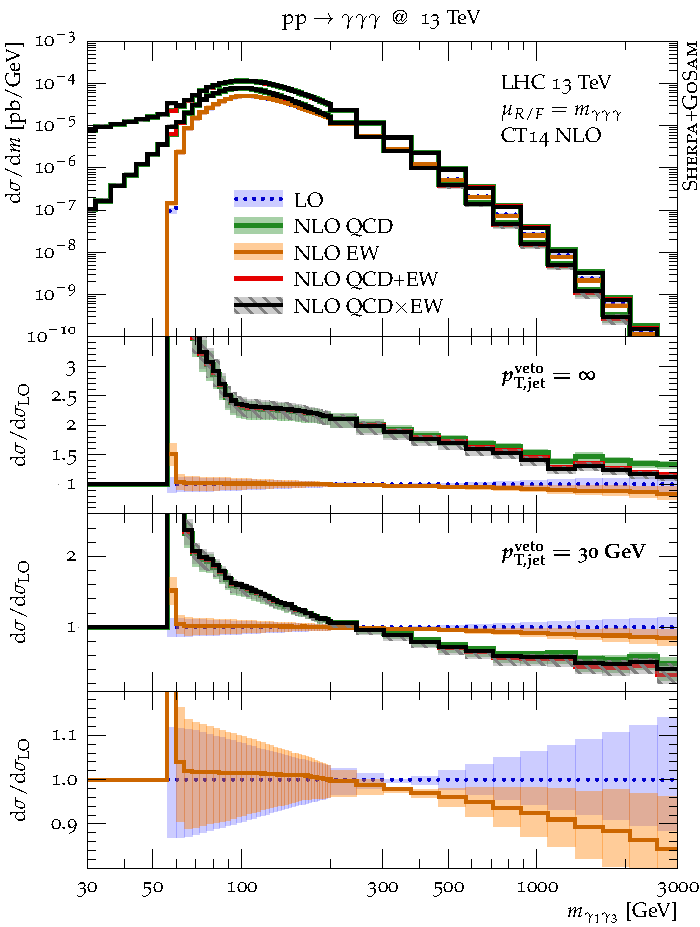
\includegraphics[width=0.32\textwidth]{figs_aaa/m_y1y3_comb_log}
  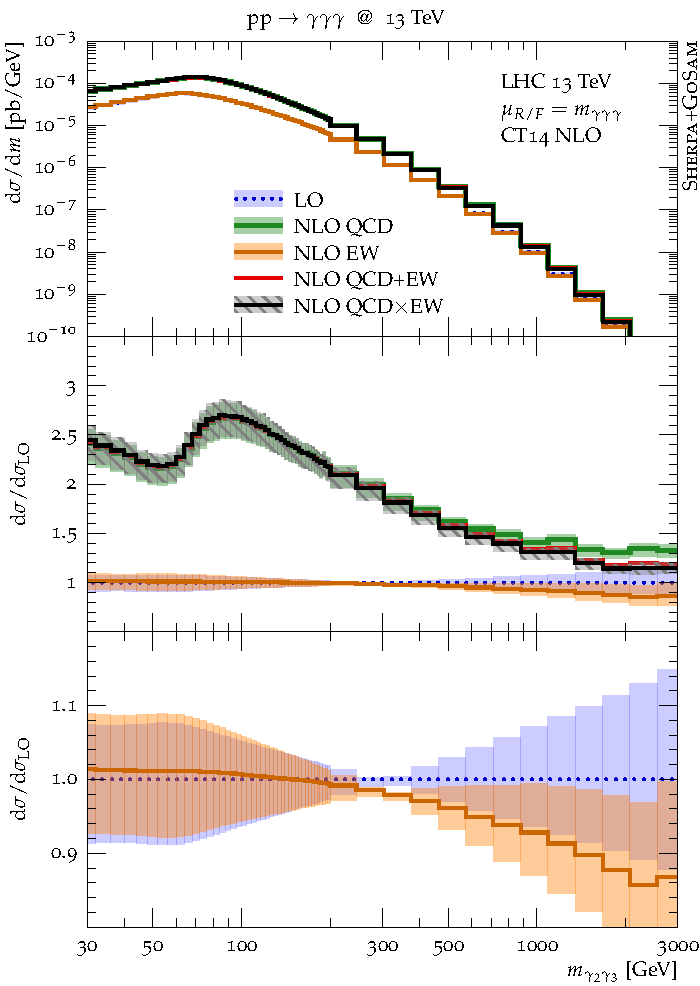
\includegraphics[width=0.32\textwidth]{figs_aaa/m_y2y3_comb_log}
  \caption{
    Pairwise invariant mass of the leading and subleading photon (left),
    leading and third leading photon (centre), subleading and third leading 
    photon (right) at the LHC at 13\,TeV.\\
    \comment{MS: Spike in $m_{\gamma_1\gamma_2}$ is in NLO \QCDtEW 
             and comes from $\deltaEW\approx 10$ in this bin at the 
             edge of the LO phase space.}
    \label{fig:aaa:myy}
  }
\end{figure}

